\subsection{Authentication}
Good security is essential in this process, as any bad actors could access sensitive information such as personal details, as well as cause havoc on the system. There is potential for one person to delay the radiology and oncology in the uk. Therefore 

We do not need CSRF tokens as ...

As seen in Figure x, all routes past the protected/ route go through the hook (which is), which checks if the user is authenticated. If they are not, they are redirected to the login page. This is done by checking the session cookie, which is set when the user logs in. This is a secure way of checking if the user is authenticated, as the session cookie is encrypted and cannot be tampered with. JWT. 

\noindent
\frame{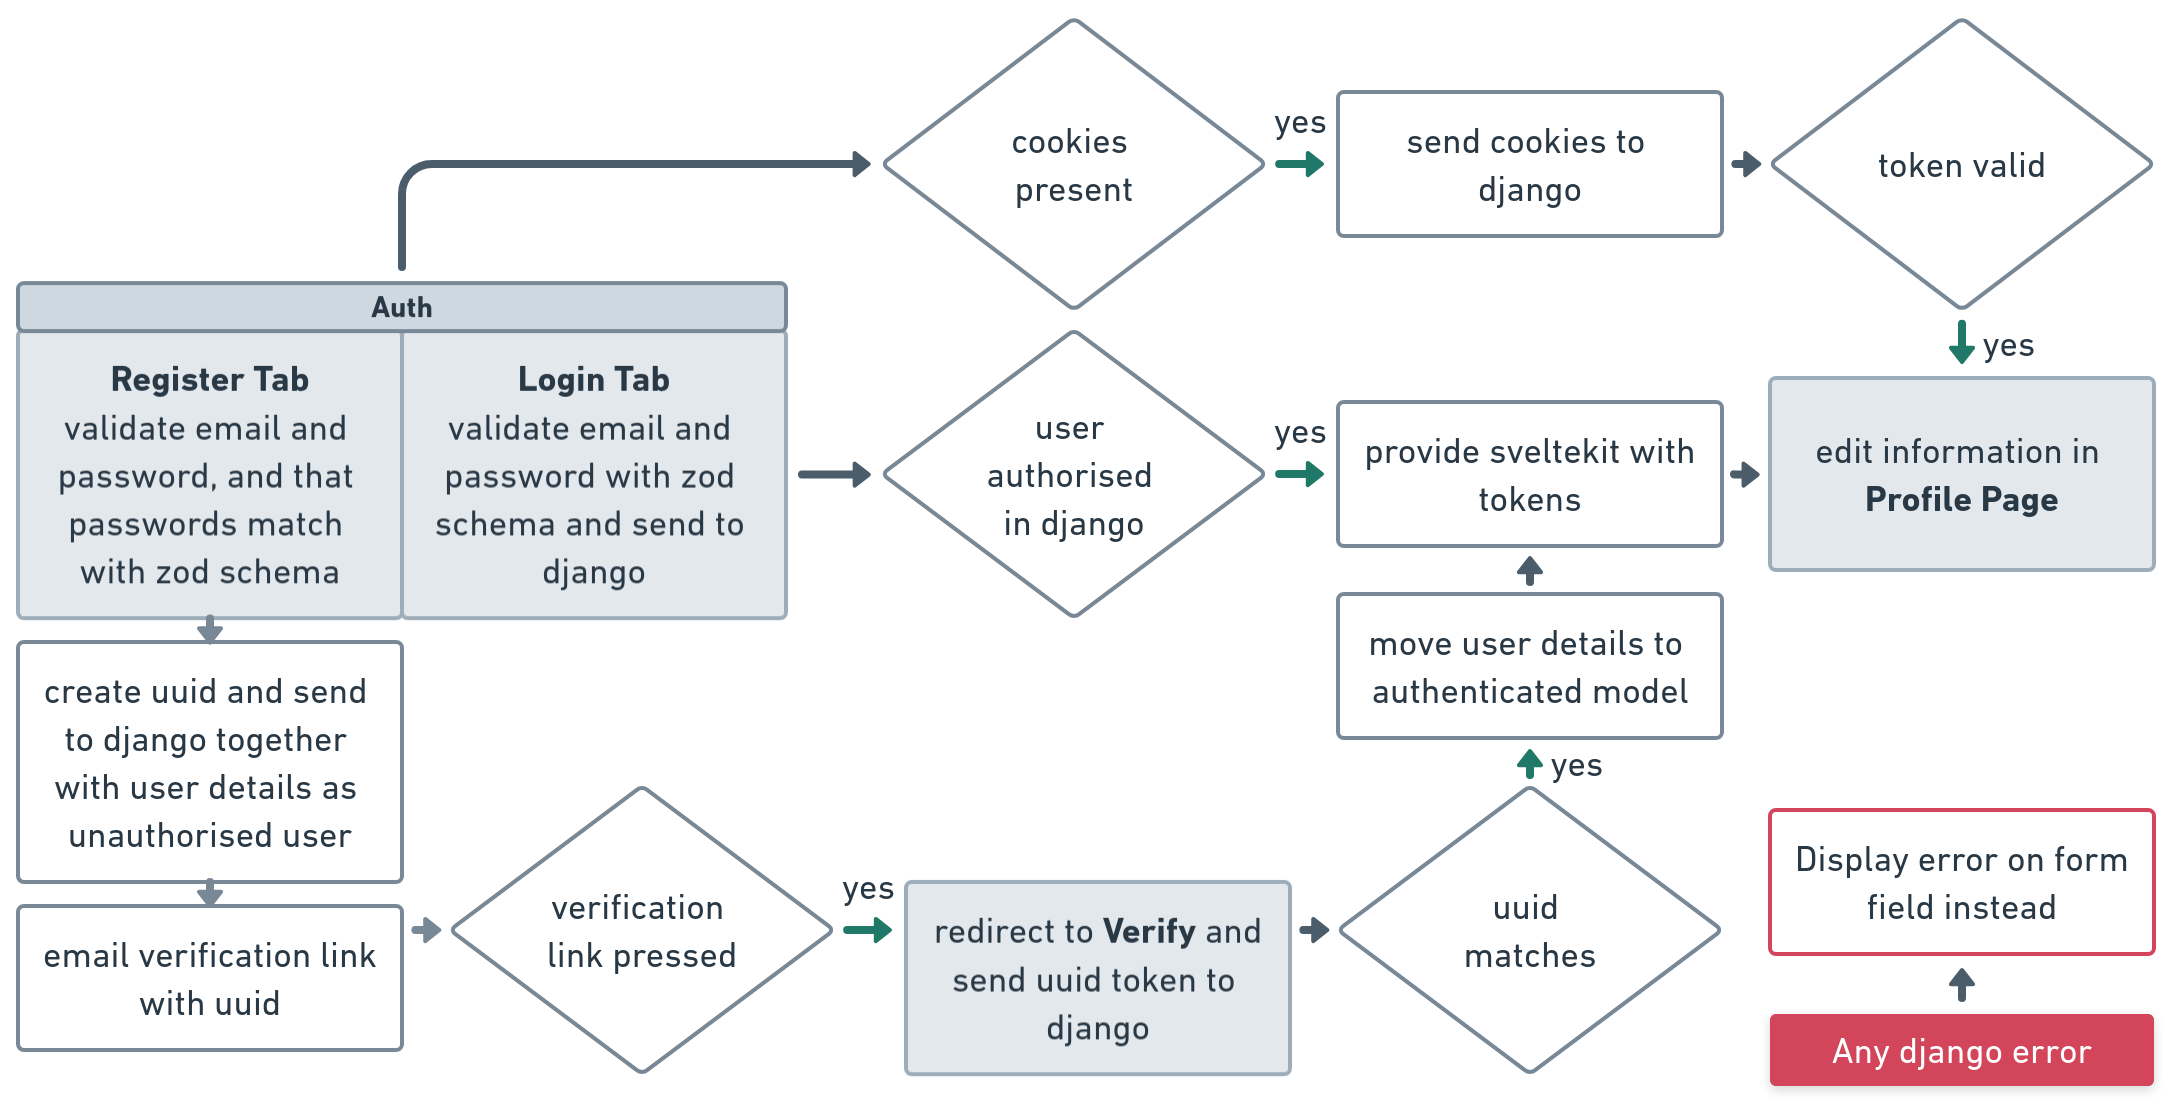
\includegraphics[width=\linewidth]{images/auth.png}}